\iffalse \bibliography{MGymrekRefs.bib} \fi

\chapter{Identifying personal genomes by surname inference}

\hzline

Most of this chapter was first published as:

\begin{itemize}

\item[] \textbf{Gymrek M}, McGuire A, Golan D, Halperin E, Erlich Y. Identifying personal genomes by surname inference. \emph{Science}. (2013).
\end{itemize}

\hzline


\textbf{Abstract:} Sharing sequencing datasets without identifiers has become a common practice in genomics. Here, we report that surnames can be recovered from personal genomes by profiling short tandem repeats on the Y-chromosome (Y-STRs) and querying recreational genetic genealogy databases. We show that a combination of a surname with other types of metadata, such as age and state, can be used to triangulate the identity of the target. A key feature of this technique is that it entirely relies on free, publicly accessible Internet resources. We quantitatively analyze the probability of identification for US males. We further demonstrate the feasibility of this technique by tracing back with high probability the identities of multiple participants in public sequencing projects.

\section{Main Text}
Surnames are paternally-inherited in most human societies, resulting in their co-segregation with Y-chromosome haplotypes \cite{SykesIrven2000,KingBallereauSchurerEtAl2006,McEvoyBradley2006,KingJobling2009,KingJobling2009a}. Based on this observation, multiple genetic genealogy companies offer services to reunite distant patrilineal relatives by genotyping a few dozen highly polymorphic short tandem repeats across the Y-chromosome (Y-STRs). The association between surnames and haplotypes can be confounded by non-paternity events, mutations, and adoption of the same surname by multiple founders \cite{KingJobling2009}. The genetic genealogy community addresses these barriers with massive databases that list the test results of Y-STR haplotypes along with their corresponding surnames. Currently, there are at least eight databases and numerous surname project websites that collectively contain hundreds of thousands surname-haplotype records (\textbf{Supplementary Table \ref{tab:sursuptab1}}). 

The ability of genetic genealogy databases to breach anonymity has been demonstrated in the past. In a number of public cases, male adoptees and descendants of anonymous sperm donors used recreational genetic genealogy services to genotype their Y-chromosome haplotypes and to search the companies' databases \cite{Lehmann-Haupt2010,Naik2009,Stein2005,Motluk2005}. The genetic matches identified distant patrilineal relatives and pointed to the potential surnames of their biological fathers. By combining other pieces of demographic information, such as date and place of birth, they fully exposed the identity of their biological fathers. Lunshof et al \cite{LunshofChadwickVorhausEtAl2008} was the first to speculate that this technique could expose the full identity of participants in sequencing projects. Gitschier \cite{Gitschier2009} empirically approached this hypothesis by testing 30 Y-STR haplotypes of CEU participants in these databases and reported that potential surnames can be detected.  [CEU participants are multigenerational familes of  northern and western European ancestry in Utah who had originally had their samples collected by CEPH (Centre d'Etude du Polymorphisme Humain) and were later reconsented to participate in the HapMap project.] However, these surnames could match thousands of individuals and full re-identification in a single person resolution was not pursued. 

Our goal was to quantitatively approach the question of how readily surname inference might be possible in a more general population, apply this approach to personal genome datasets, and demonstrate end-to-end identification of individuals using only public information. We show that full identities of personal genomes can be exposed via surname inference from recreational genetic genealogy databases followed by Internet searches. In all cases in which individuals were studied who had donated sequences, the informed consent statements they had signed stated privacy breach as a potential risk and the data usage terms did not prevent re-identification. Representatives of relevant organizations that funded the original studies were notified and confirmed the compliance of this study with their guidelines.

As a primary resource for surname inference, we focused on Ysearch (\url{www.ysearch.org}) and SMGF (\url{www.smgf.org}), the two largest public genetic genealogy databases with free-of-charge, built-in search engines. The interfaces of these engines are quite similar and allow users to insert a combination of Y-STR alleles and search for matching records based on genetic similarity. The retrieved records contain surnames typically with information about the patrilineal line, such as geographical locations, potential spelling variants, and pedigrees. In total, these databases contain 39,000 unique surname entries from approximately 135,000 records. The distribution of records per surname is significantly correlated ($R^2=0.78$, $p<1.20\times 10^{-6}$) with surname frequencies in the US, suggesting an overall good representation of this population (\textbf{Fig. \ref{fig:surfig1}A}).

To test the probability of surname inference, we challenged the two databases with an orthogonal cohort of Y-STR haplotypes consist of 34 markers (\textbf{Supplementary Table  \ref{tab:sursuptab2}}) from 911 individuals, primarily with Caucasian ancestry, whose surnames are known (\textbf{Supplementary Table  \ref{tab:sursuptab3}}). This cohort was compiled from YBase, a distinct genetic genealogy database and contains individuals with 521 surnames that segregate in the US population. In each haplotype query, our surname recovery algorithm began by retrieving the database record with the shortest Time to Most Recent Common Ancestor (TMRCA) of the input haplotype (\textbf{Supplementary Figure \ref{fig:sursup1}}, \textbf{Supplementary Table \ref{tab:sursuptab4}}). Then, it calculated a confidence score that the surname match of the retrieved record is significantly better than other matches. If the score passed a user-defined threshold, the algorithm assigned the record’s surname to the input haplotype; otherwise, it categorized it as ``unknown''. We tested the algorithm with a range of confidence thresholds to explore the trade-off between successful versus wrong recovery of surnames. Finally, we weighted the results using a stratified sampling approach to reflect the frequency of surnames in the US population (\textbf{Supplementary Material \ref{sec:sursm}}). 

Our analysis projects a success rate of approximately 12\% (s.d. 2\%) in recovering surnames of US Caucasian males (\textbf{Fig. \ref{fig:surfig1}B}, \textbf{Supplementary Figure \ref{fig:sursup2}}). This rate can be accomplished with a conservative threshold that would return a wrong surname in 5\% of cases and label 83\% of cases as unknown. Higher success rates of up to 18\% can be achieved at the price of increased probability to recover an incorrect surname. Since our input cohort is based on individuals that were tested using genetic genealogy services, our results are presumably mostly relevant to socio-economic groups with high participation in these services, namely upper and middle class US Caucasians.

Combining the recovered surname with additional demographic data can narrow down the identity of the sample originator to just a handful of individuals. The analysis above indicated that most recovered surnames are quite rare with frequencies of less than 1:4,000 of the US population, corresponding to $<$40,000 males (\textbf{Figure \ref{fig:surfig1}C}, \textbf{Supplementary Figure \ref{fig:sursup3}}) (\textbf{Supplementary Material \ref{sec:sursm}}). We considered a scenario in which the genomic data is available with the target's year of birth and state of residency, two identifiers that are not protected by the United States Health Insurance Portability and Accountability Act (HIPAA). Searching individuals by year of birth, state, and surname combinations is supported by various online public record search engines, such as PeopleFinders.com or USA-people-search.com. Based on extensive simulations with the US Census data, our results predict that year of birth and state alone are weak identifiers and searches based on their combination would match at least 60,000 US males in 50\% of cases (\textbf{Figure \ref{fig:surfig1}D}). However, when surname information is added to the search, the median list size shrinks to only 12 males, which are a few enough matches to investigate individually.

\begin{figure}[h!]
\centering
\label{fig:surfig1}
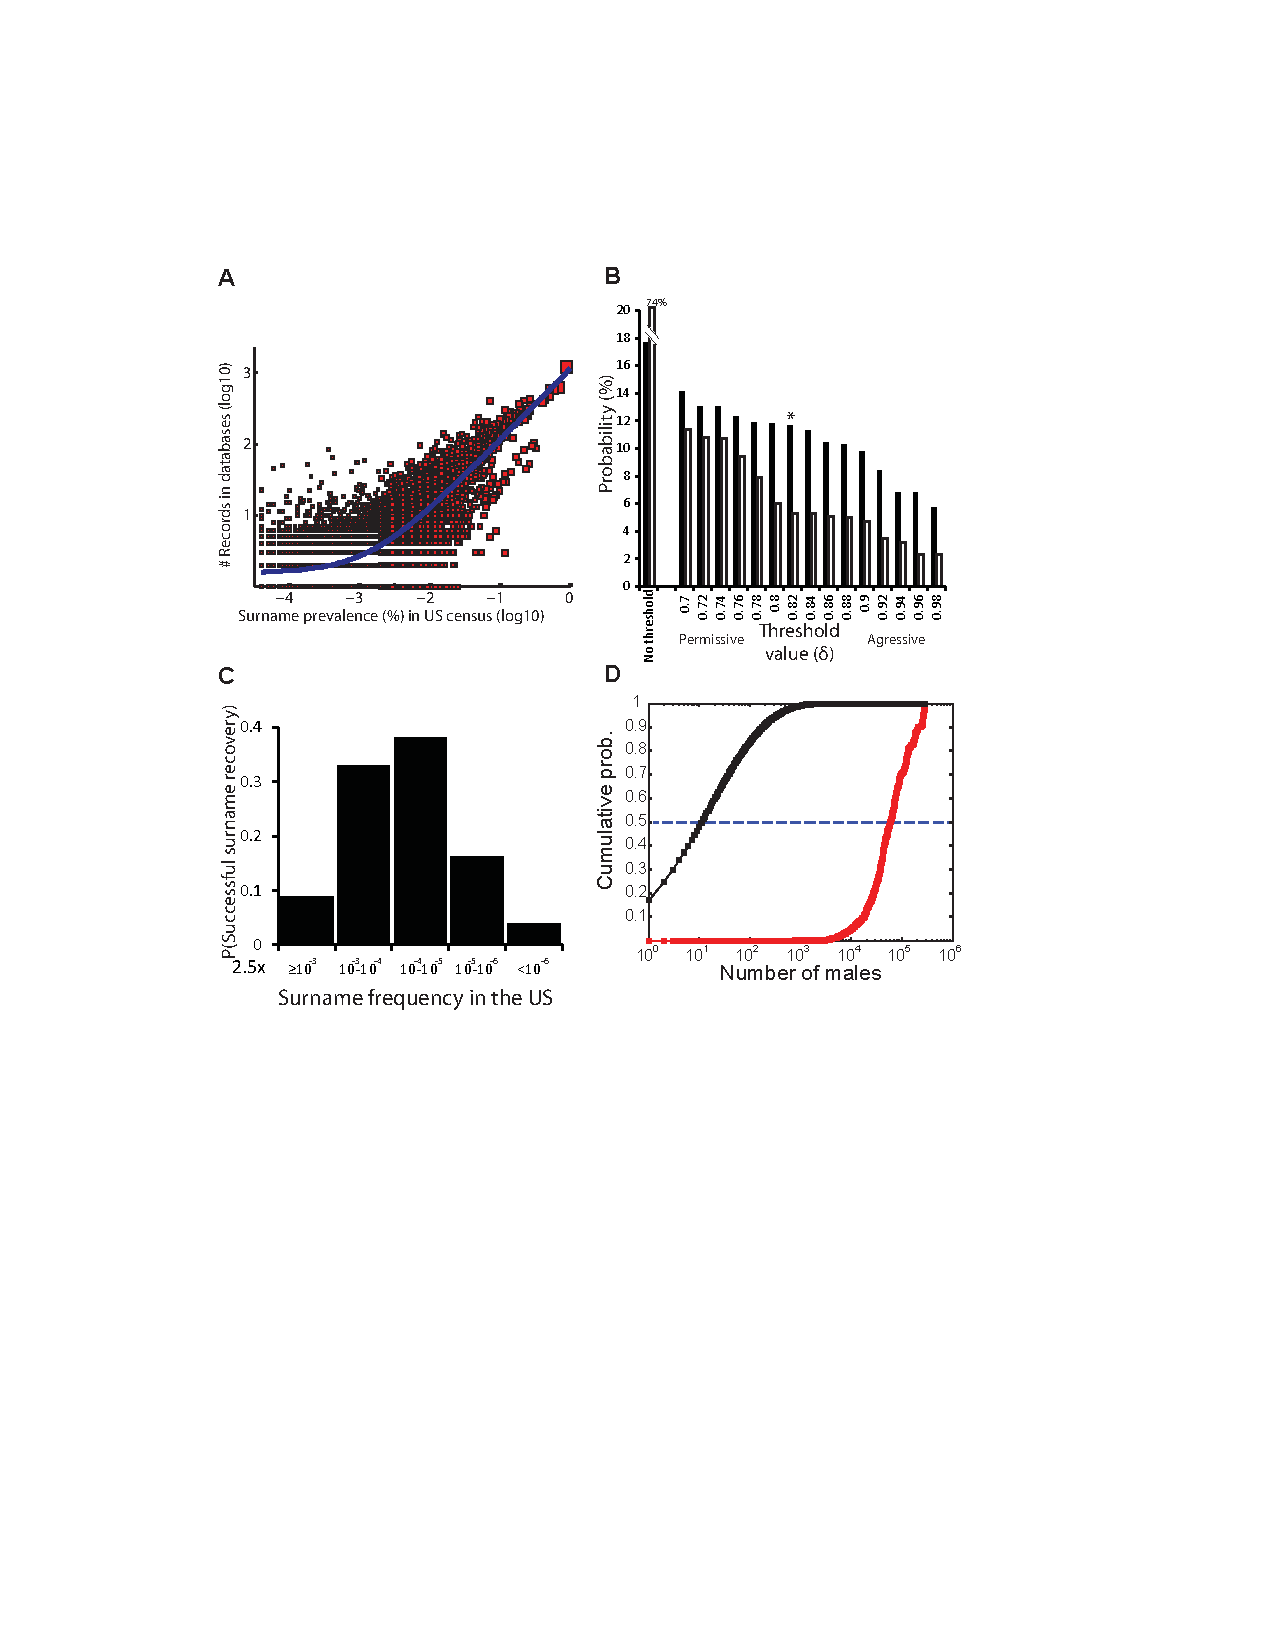
\includegraphics[width=0.5\textwidth]{Figures/App1/Fig1.pdf}
\caption{\textbf{Quantitative assessment of identification via surname inference} \textbf{(A)} The number of Ysearch and SMGF records as a function of surname prevalence in the US population. The best fit line is shown in blue. \textbf{(B)} Expected performance of surname recovery. The probability of successful recovery (closed bars) and wrong recovery (open bars) are shown at different surname confidence thresholds. The star indicates the middle-range performance threshold that was described in the main text. \textbf{(C)} The expected distribution of recovered surnames as a function of their prevalence. Most recovered surnames are expected to have a frequency of 1:4,000 individuals or less. \textbf{(D)} The cumulative distribution function of US males with a profile that matches a specific age, state, and surname combination (black) compared to the distribution when only age and state are known (red). The median is labeled with a dashed line.}
\end{figure}

Next, we established the feasibility of Illumina sequencing to produce accurate Y-STR haplotypes. Using lobSTR, an algorithm for STR profiling from raw sequencing reads \cite{GymrekGolanRossetEtAl2012}, we processed ten high coverage male genomes from the Human Genome Diversity Panel (HGDP). lobSTR produced Y-STR haplotypes with an average length of 53 out of the possible 79 genealogical markers (\textbf{Supplementary Table \ref{fig:sursup5}}). Comparing these results to capillary electrophoresis calls revealed 99\% accuracy. We further found that even at lower sequencing coverage of 10x, informative haplotypes can be obtained by lobSTR (\textbf{Supplementary Figure \ref{fig:sursup4}}). To test the ability to retrieve genetic genealogy records with the Illumina haplotypes, we profiled STRs from the genome of a US Caucasian male from our lab collection that was sequenced with Illumina 100bp reads to a coverage of 13x. In parallel, we submitted this sample to the genealogy service of Sorenson Genomics and created a Ysearch record based on their results. A search with the Illumina haplotype returned his Ysearch entry as a top record (\textbf{Supplementary Figure \ref{fig:sursup5}}).

The NCBI archives host a small number of genomes from identified individuals, providing good test cases for identification via surname inference. We used lobSTR to extract Y-STR haplotypes from the genomes of John West \cite{LeatEhrenreichBenjeddouEtAl2007}, Michael Snyder \cite{LimXueParkinEtAl2007}, and Craig Venter \cite{LevySuttonNgEtAl2007} (\textbf{Supplementary Table \ref{fig:sursup6}}). Searching Ysearch and SMGF with the Y-STR haplotypes of West and Snyder did not return their surnames and resulted in low matches to records with relatively ancient MRCAs 23-28 generations ago (\textbf{Supplementary Material \ref{sec:sursm}}). A search with Craig Venter's haplotype returned a clear match to a ``Venter'' record that was concordant at all 33 comparable markers and with an estimated TMRCA of less than 8 generations (\textbf{Figure \ref{fig:surfig2}}). We further tested whether it would be feasible to trace back Craig Venter by combining his surname with demographic profiling. A query for ``Surname: Venter, Year of Birth: 1946, State: California'' in online public record search engines retrieved two matching records of males, one of whom was Craig Venter himself. 

Surname inference from personal genomes puts the privacy of current de-identified public datasets at risk. We focused on the male genomes in the collection of Utah Residents with Northern and Western European Ancestry (CEU). The informed consent of these individuals did not definitively guarantee their privacy and stated that futuristic techniques might be able to identify them \url{http://hapmap.ncbi.nlm.nih.gov/downloads/elsi/CEPH_Reconsent_Form.pdf}. To test the ability to trace back the identities of these samples from personal genomes, we processed with lobSTR 32 Illumina genomes of CEU male founders that reside in public repositories of the 1000 Genomes Project \cite{AbecasisAltshulerAutonEtAl2010} and the European Nucleotide Archive that were sequenced with read lengths of at least 76bp. Most of these genomes were sequenced to a shallow depth of less than 5x, and produced sparse Y-STR haplotypes. We selected the ten genomes that had the longest Y-STR haplotypes with a range of 34-68 markers to attempt surname recovery. Searching the genetic genealogy databases returned top-matching records with Mormon ancestry in 8 of the 10 individuals for which the top hit had at least 12 comparable markers. Moreover, for four individuals, the top match consisted of multiple records with the same surname, increasing the confidence that the correct surname was retrieved. This potential high surname recovery rate stems from a combination of the deep interest in genetic genealogy among this population and the large family sizes, which exponentially increases the number of targeted individuals for every person that is tested. 

\begin{figure}[h!]
\centering
\label{fig:surfig2}
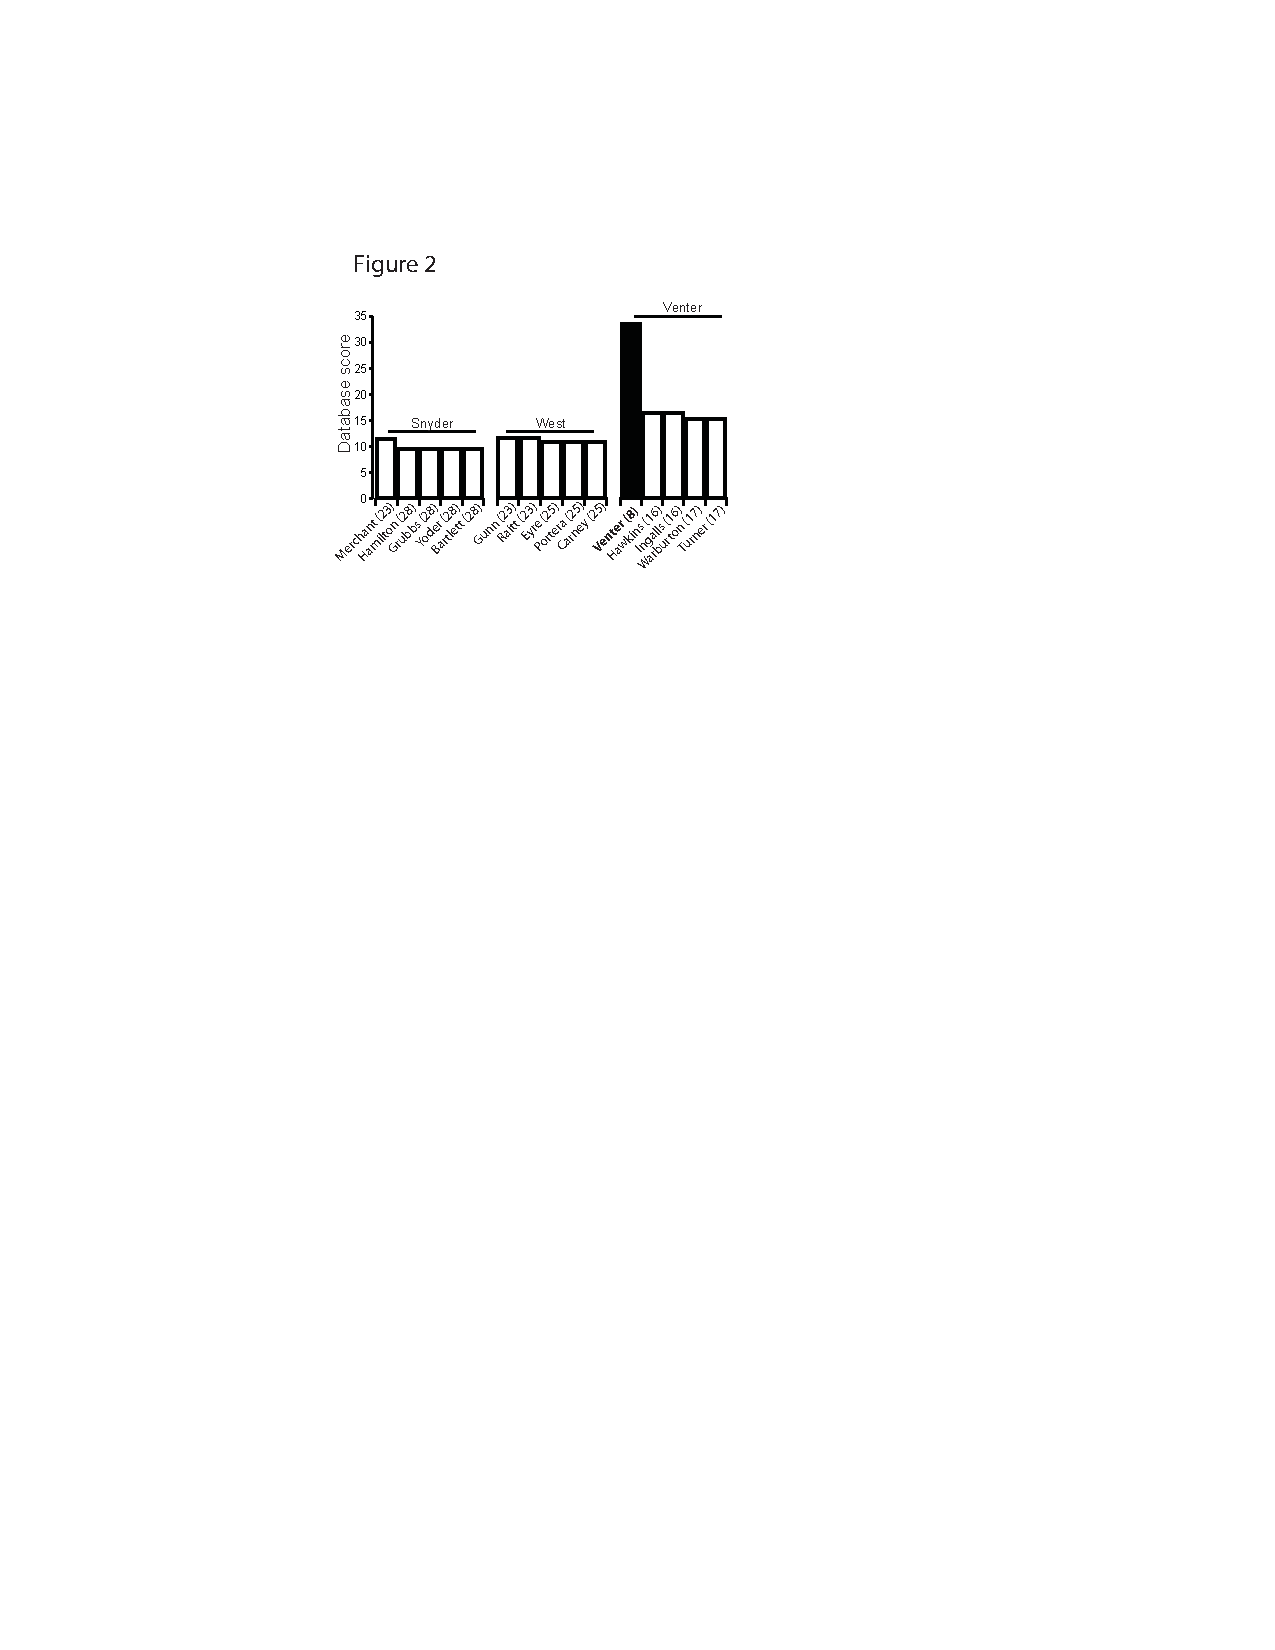
\includegraphics[width=0.5\textwidth]{Figures/App1/Fig2.pdf}
\caption{\textbf{The top five records retrieved after searching Ysearch with the Y-STR haplotypes of Michael Snyder, John West, and Craig Venter.} The expected number of generations to the MRCA is given in parentheses for each record. Searching with Craig Venter returned a ``Venter'' record (closed bar) as the top match.}
\end{figure}

In five surname recovery cases, we fully identified the CEU individuals and their entire families with very high probabilities (\textbf{Table \ref{tab:surtab1}}). These five cases belonged to three pedigrees, where in two of these pedigrees the surnames of both the paternal and maternal grandfathers were recovered. Our strategy for tracing back individuals relied on the recovered surnames as well as publicly available Internet resources such as record search engines, obituaries, and genealogical websites, and demographic metadata available in the Coriell Cell Repository website. The year of birth was inferred by subtracting the ages in Coriell from the year of collecting samples. Each search took 3 to 7 hours by a single person. The identified families matched exactly to the corresponding pedigree descriptions in the Coriell database: the number of children, the birth order of daughters and sons, and the state of residence were identical. All grandparents were alive in 1984, the year that the CEU cell line collection was established \cite{PrescottLalouelLeppert2008}. In the two cases of a dual surname recovery from both grandfathers, the surname of the father and the maiden name of the mother matched exactly to the grandfathers' surnames, substantially increasing the confidence of the recovery. Coriell also lists the ages during sample collection for these two pedigrees, which agreed with the age differences of the identified family members. Using genealogical websites, we traced the patrilineal lineage that connects each identified genome through the MRCA to the record originator in the genetic genealogy database (\textbf{Fig. \ref{fig:surfig3}}). This analysis revealed that two to seven meiosis events link the CEU genome to the record source. Finally, we calculated that the probability of finding random families in the Utah population with these exact demographic characteristics is less than 1 in 105-109 (\textbf{Supplementary Material \ref{sec:sursm}}). In total, surname inference breached the privacy of nearly 50 individuals from these three pedigrees.

This study shows that data release, even of a few markers, by one person can spread through deep genealogical ties and lead to the identification of another person who might have no acquaintance with the person who released his genetic data. The propagation of information through shared male lines amplifies the range of identification, allowing $\sim$135,000 records to potentially target several millions of US males. Another feature of this identification technique is that it entirely relies on free, publicly-available resources. It can be completed end-to-end with only computational tools and an Internet connection. The compatibility of our technique with public record search engines makes it much easier to continue identifying other datasets in the same pedigree, including female genomes, once one male target is identified.  We envision that the risk of surname inference will grow in the future. Genetic genealogy enthusiasts add thousands of records to these databases every month. In addition, the advent of third-generation sequencing platforms with longer reads will enable even higher coverage of Y-STR markers, further strengthening the ability to link haplotypes and surnames.

\begin{figure}[h!]
\centering
\label{fig:surfig3}
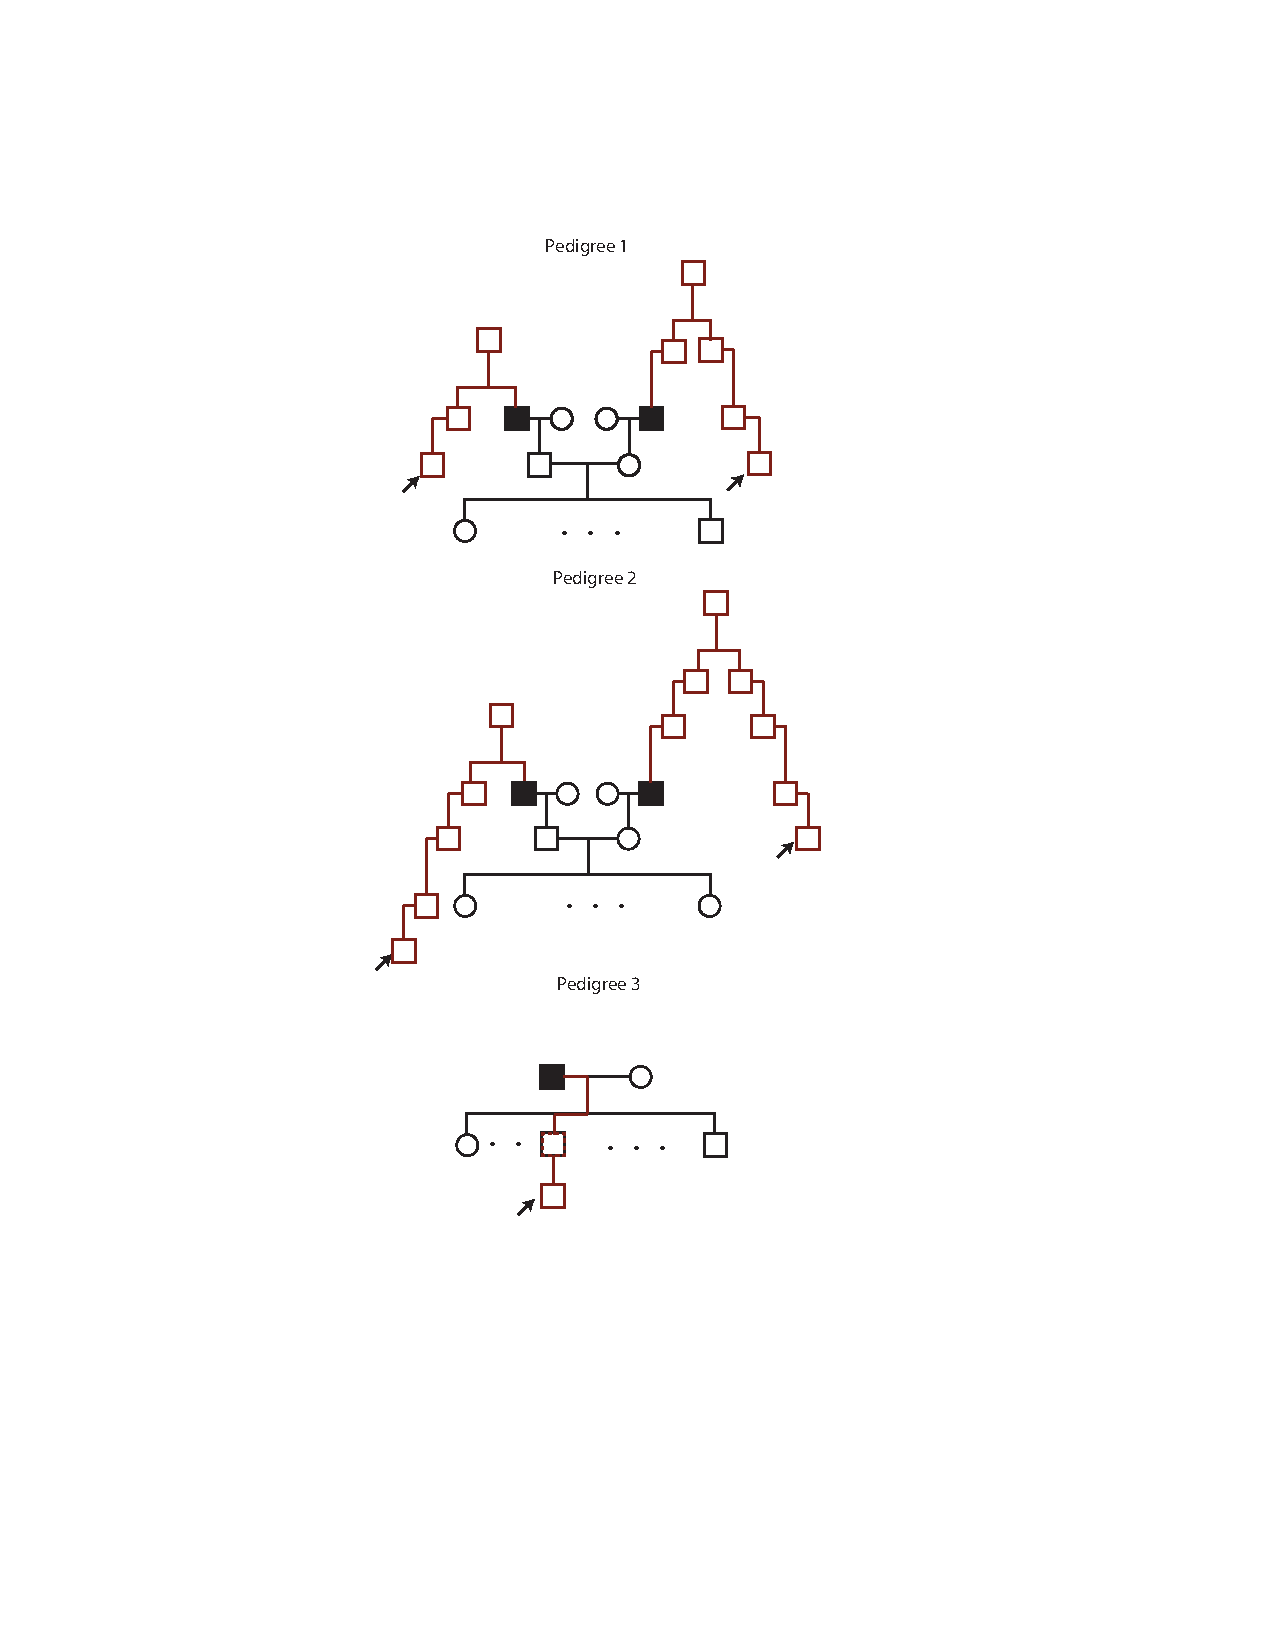
\includegraphics[width=0.5\textwidth]{Figures/App1/Fig3.pdf}
\caption{\textbf{Illustrations of the three CEU pedigrees (black) showing how genetic information from distant patrilineal relatives (arrow; red - patrilineal lines) can identify individuals.} Filled rectangles represent sequenced individuals. To respect the privacy of these families, only abbreviated versions are presented. The sex of the CEU grandchildren was randomized.  The numbers of grandchildren are not given.}
\end{figure}

Similar to other genetic privacy issues \cite{LinOwenAltman2004,BieberBrennerLazer2006,HomerSzelingerRedmanEtAl2008,JacobsYeagerWacholderEtAl2009,ImGamazonNicolaeEtAl2012,CraigGoorWangEtAl2011,SchadtWooHao2012}, preventing surname inference from public whole genome datasets might be quite challenging. Masking Y-STR markers could limit the effectiveness of the method presented in this study, but this approach is not sustainable (\textbf{Supplementary Material \ref{sec:sursm}}). Our analysis suggests that Y-STR haplotypes can be imputed back from SNPs on the Y-chromosome (Y-SNPs) when a large reference set of male genomes will be available (\textbf{Supplementary Figure \ref{fig:sursup6}}). In addition, community efforts, such as the Y Chromosome Genome Comparison, have already started exploring the association between Y-SNPs and surnames (\textbf{Supplementary Table \ref{tab:sursuptab1}}), and might allow bypassing Y-STR masking. We also posit that restricting genetic genealogy information is not practical as some of the data is already scattered in multiple end-user websites and genealogy mailing lists. 

Existing policy tools, such as controlled access databases with data use agreements, may mediate the exposure of genomic information to surname inference. However, in our view, the appropriate response to genetic privacy challenges such as these is not for the public to stop donating samples or for data sharing to stop - which would be devastating reactions that could significantly hamper scientific progress. Rather, we believe that establishing clear policies for data sharing, educating participants about the benefits and risks of genetic studies \cite{McGuireGibbs2006} and the legislation of proper usage of genetic information are pivotal ingredients to support the genomic endeavor.

\begin{figure}[h!]
\centering
\label{tab:surtab1}
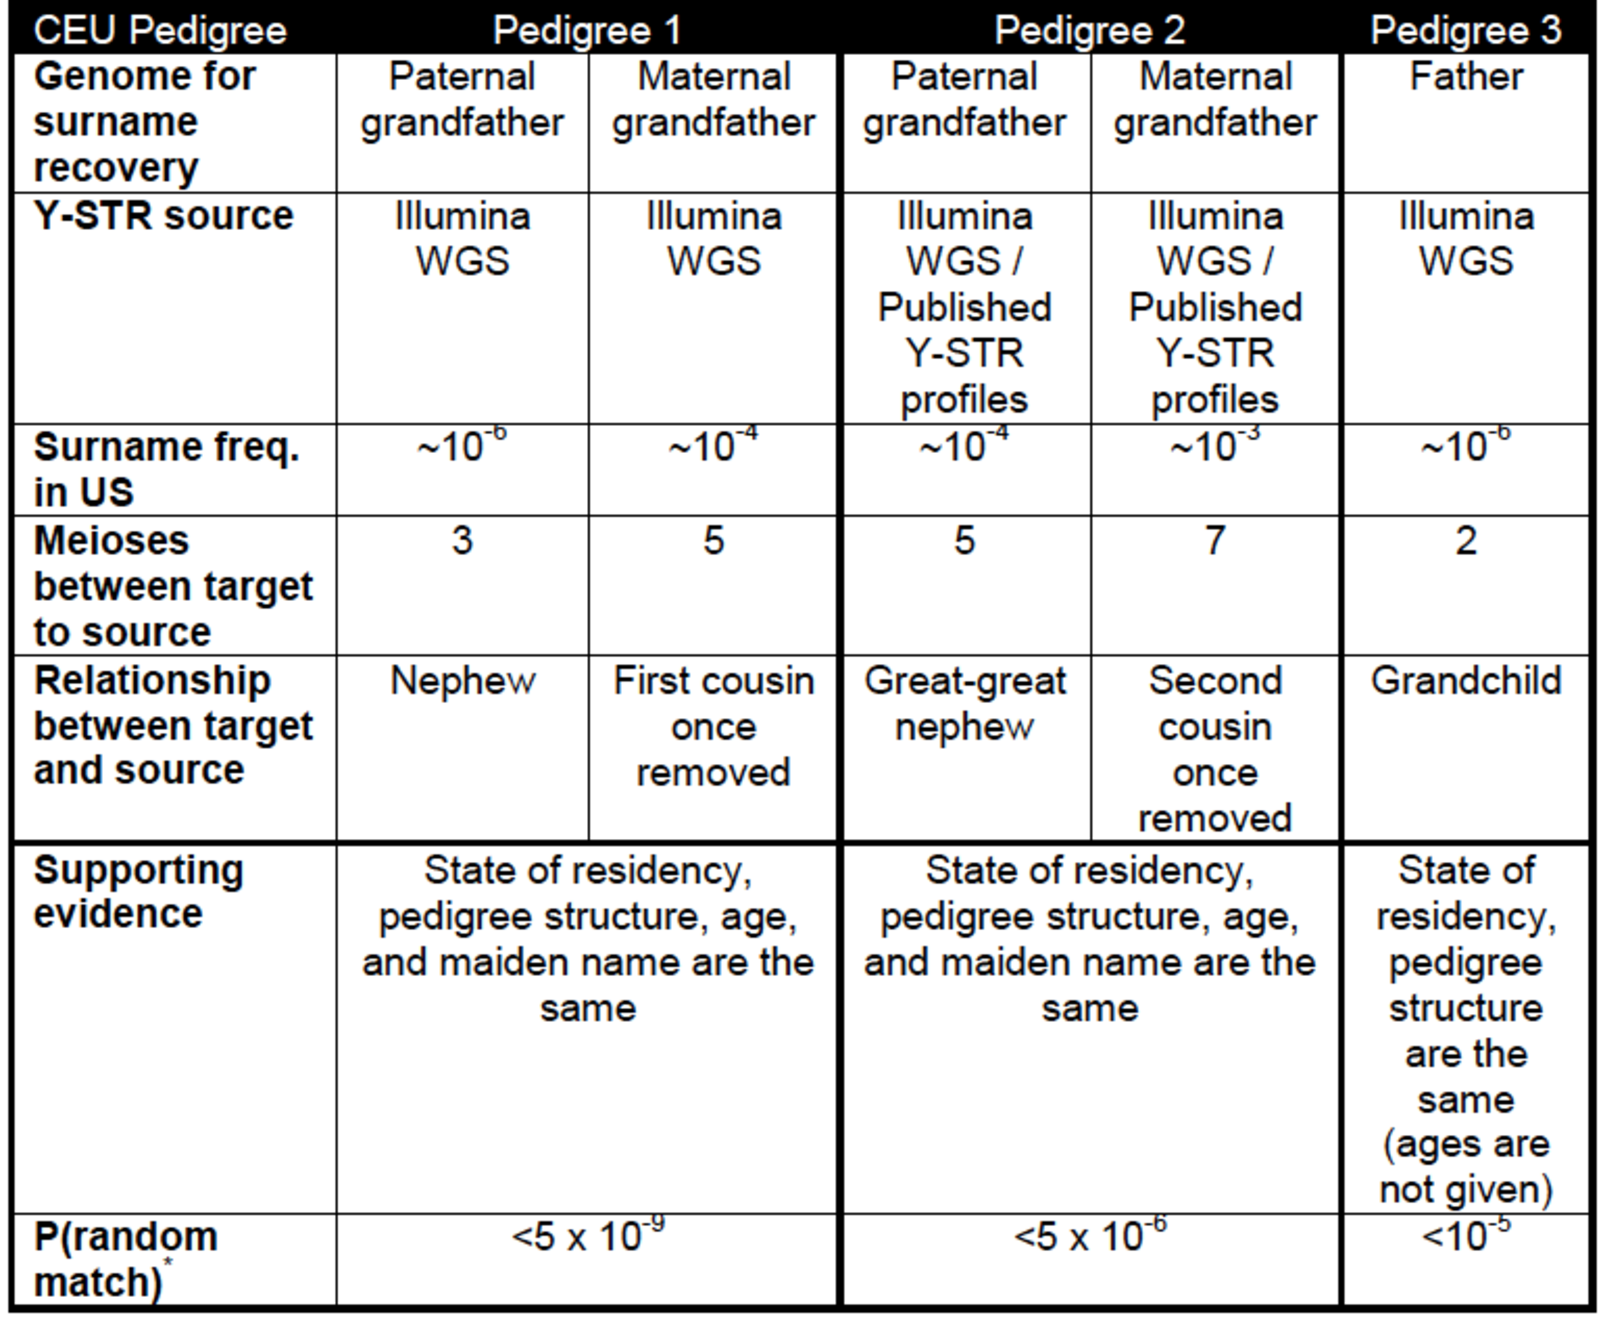
\includegraphics[width=0.9\textwidth]{Figures/App1/Table1.pdf}
\caption{\textbf{Comparison of CEU identification cases.}}
\end{figure}

\section{Supplementary Material}
\label{sec:sursm}

\pagebreak
\section{Supplemental Figures}
\subsection{Supplemental Figure 1}
\begin{figure}[h!]
\centering
\label{fig:sursup1}
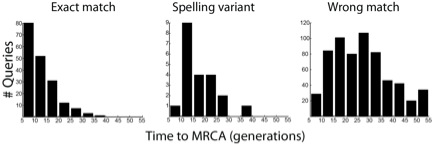
\includegraphics[width=0.65\textwidth]{Figures/App1/SuppFig1.jpg}
\end{figure}
\textbf{The TMRCA profiles of haplotype queries.} Records that matched exactly the input surname (left) showed a geometric-like distribution. For most records with a minute spelling variant from the original surname (center) the  MRCA was 10-15 generations ago. Wrong matches (right) mainly showed an ancient MRCA.

\pagebreak
\subsection{Supplemental Figure 2}
\begin{figure}[h!]
\centering
\label{fig:sursup2}
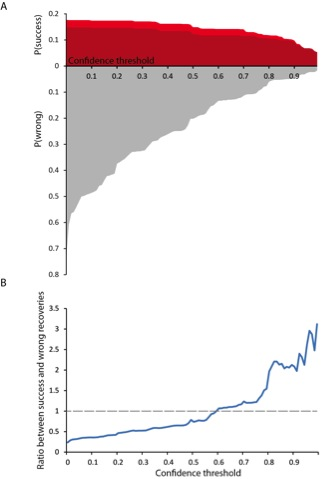
\includegraphics[width=0.4\textwidth]{Figures/App1/SuppFig2.jpg}
\end{figure}
\textbf{Performance of surname recovery at different confidence thresholds.} \textbf{(A)} The rate of successful recovery with exact matches (dark red) and spelling variants (light red) versus the wrong recovery rate (gray) as a function of confidence threshold level. \textbf{(B)} The ratio between successful recoveries to wrong recoveries.

\pagebreak
\subsection{Supplemental Figure 3}
\begin{figure}[h!]
\centering
\label{fig:sursup3}
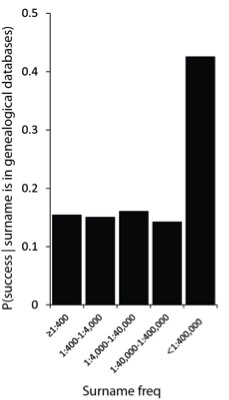
\includegraphics[width=0.4\textwidth]{Figures/App1/SuppFig3.jpg}
\end{figure}
\textbf{The probability of successful recovery given that the surname has at least one record in Ysearch or SMGF as a function of the surname frequency.}

\pagebreak
\subsection{Supplemental Figure 4}
\begin{figure}[h!]
\centering
\label{fig:sursup4}
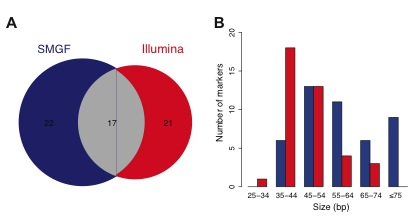
\includegraphics[width=0.65\textwidth]{Figures/App1/SuppFig4.jpg}
\end{figure}
\textbf{Comparison between Illumina Y-STR profiling and the Sorenson Genomics genetic genealogy service.} \textbf{(A)} Illumina profiling returned the results of 38 Y-STR markers. The genetic genealogy service uses a panel of 49 markers, 39 of which are included in lobSTR’s Y-STR reference. The results of all 17 markers that were profiled by both strategies were identical. \textbf{(B)} The distribution of total STR region lengths is shown for the markers typed by Sorenson (blue) versus markers typed by lobSTR (red).

\pagebreak
\subsection{Supplemental Figure 5}
\begin{figure}[h!]
\centering
\label{fig:sursup5}
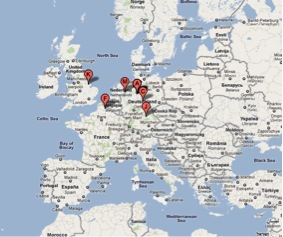
\includegraphics[width=0.65\textwidth]{Figures/App1/SuppFig5a.jpg}
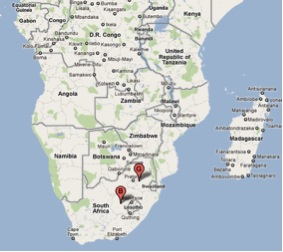
\includegraphics[width=0.65\textwidth]{Figures/App1/SuppFig5b.jpg}
\end{figure}
\textbf{Ancestral origins of Venter records in Ysearch}. The ancestral origin of the top match is labeled with an arrow.

\pagebreak
\subsection{Supplemental Figure 6}
\begin{figure}[h!]
\centering
\label{fig:sursup6}
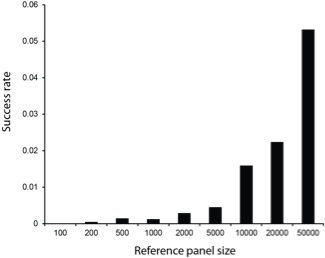
\includegraphics[width=0.65\textwidth]{Figures/App1/SuppFig6.jpg}
\end{figure}
\textbf{The estimated success rate for surname recovery after imputation as a function of the imputation panel size.}

\pagebreak
\section{Supplemental Tables}
\subsection{Supplemental Table 1}
\begin{figure}[h!]
\centering
\label{tab:sursuptab1} % even though we use a figure screenshot
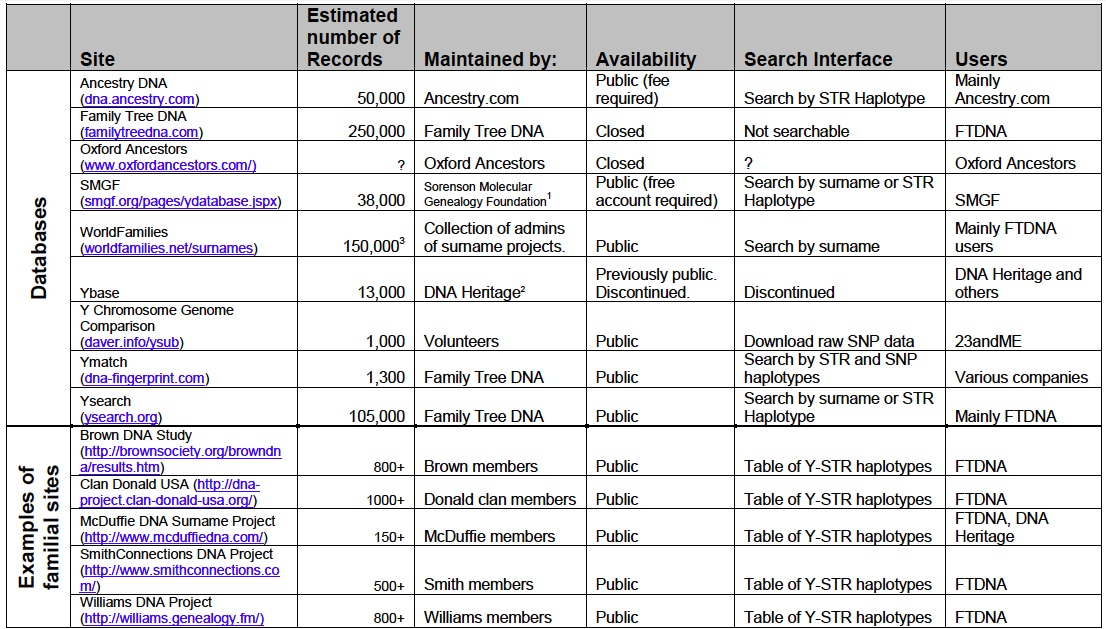
\includegraphics[width=0.95\textwidth]{Figures/App1/SuppTab1.jpg}
\end{figure}
List of major genetic genealogy sites that display Y chromosome and surname information. The top section lists genetic genealogy databases. The bottom section lists examples of privately maintained familial genetic genealogy sites.
$^1$ SMGF was recently acquired by Ancestry.com. $^2$ DNA Heritage was acquired by FamilyTreeDNA in 2011. $^3$ Includes only users whose surnames are present in the 2000 US Census.

\pagebreak
\subsection{Supplemental Table 2}
\begin{table}[h!]
\centering
\label{tab:sursuptab2}
\begin{adjustbox}{height=0.4\textheight}
\begin{tabular}{l l l l}
\hline
Marker & Expected mutation rate & Mean & $\sigma$ \\
\hline
DYS19     & 0.00437  & 14.34   & 0.8045 \\
DYS385a   & 0.00208  & 12.0869 & 1.6522 \\
DYS385b   & 0.00414  & 14.5464 & 1.449  \\
DYS388    & 0.000425 & 12.5142 & 1.0753 \\
DYS389a   & 0.00551  & 12.9668 & 0.6644 \\
DYS389b   & 0.00383  & 29.326  & 1.0418 \\
DYS390    & 0.00152  & 23.6032 & 1.0229 \\
DYS391    & 0.00323  & 10.4858 & 0.6104 \\
DYS392    & 0.00097  & 12.3413 & 1.1069 \\
DYS393    & 0.00211  & 13.0752 & 0.6025 \\
DYS426    & 0.000398 & 11.6459 & 0.5198 \\
DYS437    & 0.00153  & 14.9094 & 0.6931 \\
DYS438    & 0.000956 & 11.2206 & 1.0643 \\
DYS439    & 0.00384  & 11.66   & 0.8567 \\
DYS442    & 0.00978  & 17.2273 & 1.3301 \\
DYS444    & 0.00545  & 12.3666 & 0.892  \\
DYS445    & 0.00216  & 11.6015 & 0.9401 \\
DYS446    & 0.00267  & 13.1767 & 1.372  \\
DYS447    & 0.00212  & 24.6396 & 1.2057 \\
DYS448    & 0.000394 & 19.3437 & 0.8748 \\
DYS449    & 0.0122   & 29.5472 & 1.6474 \\
DYS452    & 0.00402  & 30.1854 & 1.1041 \\
DYS454    & 0.000475 & 11.0484 & 0.3744 \\
DYS455    & 0.000426 & 10.648  & 0.9704 \\
DYS456    & 0.00494  & 15.4571 & 1.1065 \\
DYS458    & 0.00836  & 16.6389 & 1.2634 \\
DYS459a   & 0.00013  & 8.753   & 0.5017 \\
DYS459b   & 0.00013  & 9.601   & 0.5422 \\
DYS460    & 0.00622  & 10.6976 & 0.639  \\
DYS461    & 0.000989 & 11.882  & 0.6914 \\
DYS462    & 0.00265  & 11.3571 & 0.6266 \\
DYS464a   & 0.00018  & 13.8555 & 1.4488 \\
DYS464b   & 0.00018  & 14.7374 & 1.0564 \\
DYS464c   & 0.00018  & 15.8236 & 1.124  \\
DYS464d   & 0.00018  & 16.5742 & 1.1157 \\
DYS635    & 0.00385  & 22.6604 & 1.1601 \\
GATA-A10  & 0.00332  & 15.5234 & 1.2242 \\
GATA-H4   & 0.00322  & 10.7333 & 0.7801 \\
GGAAT1B07 & 0.0024   & 10.2854 & 0.7397 \\
YCAIIa    & 0.002    & 19.0997 & 0.905  \\
YCAIIb    & 0.002    & 22.136  & 1.2624 \\
\hline
\end{tabular}
\end{adjustbox}
\caption{\textbf{List of markers used to challenge Ysearch and SMGF.} Mutation rates are based on Ballantyne et al. \cite{BallantyneGoedbloedFangEtAl2010}. YCAII was absent from this study and set to 0.002 according to Walsh \cite{Walsh2001}. Mean and standard deviations for marker values are calculated using Ysearch with NIST nomenclature.}
\end{table}

\pagebreak
\subsection{Supplemental Table 3}
\label{tab:sursuptab3}
\begin{tabularx}{\linewidth}{l l l l l l }
\hline
Marker & Start & End & Alt location & Ref allele & Motif structure \\
\hline
DYS394/19   & 9521989  & 9522052  &                        & 15 & {[}TAGA{]}3TAGG{[}TAGA{]}n                                                                                                           \\
DYS385a/b   & 20842518 & 20842573 & chrY:19260956-19261212 & 14 & {[}GAAA{]}n                                                                                                                          \\
DYS388      & 14747535 & 14747570 &                        & 12 & {[}ATT{]}n                                                                                                                           \\
DYS389I     & 14612191 & 14612238 &                        & 12 & {[}TCTG{]}m{[}TCTA{]}n                                                                                                               \\
DYS389B     & 14612338 & 14612405 &                        & 29 & {[}TCTG{]}m{[}TCTA{]}n                                                                                                               \\
DYS390      & 17274947 & 17275042 &                        & 24 & {[}TCTG{]}n{[}TCTA{]}m{[}TCTG{]}p{[}TCTA{]}q                                                                                         \\
DYS391      & 14102795 & 14102838 &                        & 11 & {[}TCTA{]}n                                                                                                                          \\
DYS392      & 22633873 & 22633911 &                        & 13 & {[}TAT{]}n                                                                                                                           \\
DYS393      & 3131152  & 3131199  &                        & 12 & {[}AGAT{]}n                                                                                                                          \\
DYS406S1    & 23843595 & 23843634 &                        & 10 & {[}TATC{]}n                                                                                                                          \\
DYS413a/b   & 16099088 & 16099133 & chrY:14676647-14676820 & 23 & {[}TG{]}n                                                                                                                            \\
DYS426      & 19134850 & 19134885 &                        & 12 & {[}GTT{]}n                                                                                                                           \\
DYS434      & 14466533 & 14466568 &                        & 9  & TAAT{[}CTAT{]}n                                                                                                                      \\
DYS435      & 14496298 & 14496333 &                        & 9  & {[}TGGA{]}n                                                                                                                          \\
DYS436      & 15203862 & 15203897 &                        & 12 & {[}GTT{]}n                                                                                                                           \\
DYS437      & 14466994 & 14467057 &                        & 16 & {[}TCTA{]}n{[}TCTG{]}2{[}TCTA{]}4                                                                                                    \\
DYS438      & 14937824 & 14937873 &                        & 10 & {[}TTTTC{]}n                                                                                                                         \\
DYS439      & 14515312 & 14515363 &                        & 13 & {[}GATA{]}n                                                                                                                          \\
DYS441      & 14981831 & 14981908 &                        & 16 & {[}TTCC{]}n                                                                                                                          \\
DYS442      & 14761103 & 14761168 &                        & 17 & {[}TATC{]}2{[}TGTC{]}3{[}TATC{]}n                                                                                                    \\
DYS444      & 19226192 & 19226247 &                        & 14 & {[}TAGA{]}n                                                                                                                          \\
DYS445      & 22092602 & 22092649 &                        & 12 & {[}TTTA{]}n                                                                                                                          \\
DYS446      & 3131458  & 3131527  &                        & 14 & {[}TCTCT{]}n                                                                                                                         \\
DYS447      & 15278740 & 15278854 &                        & 23 & {[}TAATA{]}n{[}TAAAA{]}1{[}TAATA{]}m{[}TAAAA{]}1{[}TAATA{]}p                                                                         \\
DYS448\_1   & 24365070 & 24365136 &                        & 11 & {[}AGAGAT{]}n                                                                                                                        \\
DYS448\_2   & 24365178 & 24365225 &                        & 8  & {[}AGAGAT{]}n                                                                                                                        \\
DYS449\_1   & 8218014  & 8218074  &                        & 13 & {[}TTTC{]}n                                                                                                                          \\
DYS449\_2   & 8218124  & 8218179  &                        & 14 & {[}TTTC{]}n                                                                                                                          \\
DYS450      & 8126300  & 8126344  &                        & 8  & {[}ATTTT{]}n                                                                                                                         \\
DYS452      & 21620478 & 21620632 &                        & 31 & {[}TATAC{]}m{[}TGTAC{]}n{[}TATAC{]}p{[}CATAC{]}{[}TATAC{]}{[}CATAC{]}{[}TATAC{]}q{[}CATAC{]}r{[}TATAC{]}s{[}CATAC{]}{[}TATAC{]}t     \\
DYS454      & 8224156  & 8224199  &                        & 11 & {[}AAAT{]}n                                                                                                                          \\
DYS455      & 6911569  & 6911612  &                        & 11 & {[}AAAT{]}n                                                                                                                          \\
DYS456      & 4270960  & 4271019  &                        & 15 & {[}AGAT{]}n                                                                                                                          \\
DYS458      & 7867880  & 7867943  &                        & 16 & {[}GAAA{]}n                                                                                                                          \\
DYS459a/b   & 26078851 & 26078890 & chrY:26292857-26293004 & 10 & {[}TAAA{]}n                                                                                                                          \\
DYS460      & 21050842 & 21050881 &                        & 10 & {[}ATAG{]}n                                                                                                                          \\
DYS461      & 21050690 & 21050737 &                        & 12 & {[}TAGA{]}n{[}CAGA{]}                                                                                                                \\
DYS462      & 21317047 & 21317090 &                        & 11 & {[}TATG{]}n                                                                                                                          \\
DYS463      & 7643509  & 7643628  &                        & 24 & {[}AAAGG{]}m {[}AAGGG{]}n {[}AAGGA{]}p                                                                                               \\
DYS472      & 16508484 & 16508507 &                        & 8  & {[}AAT{]}n                                                                                                                           \\
DYS481      & 8426378  & 8426443  &                        & 22 & {[}CTT{]}n                                                                                                                           \\
DYS485      & 22099634 & 22099681 &                        & 16 & {[}TTA{]}n                                                                                                                           \\
DYS487      & 8914174  & 8914212  &                        & 13 & {[}TTA{]}n                                                                                                                           \\
DYS490      & 3443765  & 3443800  &                        & 12 & {[}TTA{]}n                                                                                                                           \\
DYS492      & 17414337 & 17414369 &                        & 12 & {[}ATT{]}n                                                                                                                           \\
DYS494      & 21386168 & 21386197 &                        & 10 & {[}TTA{]}n                                                                                                                           \\
DYS495      & 15011300 & 15011346 &                        & 15 & {[}AAT{]}n                                                                                                                           \\
DYS505      & 3640831  & 3640878  &                        & 12 & {[}TCCT{]}n                                                                                                                          \\
DYS511      & 17304923 & 17304958 &                        & 10 & {[}GATA{]}n                                                                                                                          \\
DYS520      & 7730432  & 7730511  &                        & 20 & {[}ATAG{]}n{[}ATAC{]}n                                                                                                               \\
DYS522      & 7415625  & 7415664  &                        & 10 & {[}GATA{]}n                                                                                                                          \\
DYS531      & 8466195  & 8466238  &                        & 11 & {[}AAAT{]}n                                                                                                                          \\
DYS533      & 18393226 & 18393273 &                        & 12 & {[}ATCT{]}n                                                                                                                          \\
DYS634      & 18392976 & 18393035 &                        & 15 & {[}CTTT{]}n                                                                                                                          \\
DYS537      & 19358850 & 19358889 &                        & 10 & {[}TCTA{]}n                                                                                                                          \\
DYS549      & 21520224 & 21520275 &                        & 13 & {[}GATA{]}n                                                                                                                          \\
DYS556      & 22601453 & 22601496 &                        & 11 & {[}AATA{]}n                                                                                                                          \\
DYS557      & 23234712 & 23234775 &                        & 16 & {[}TTTC{]}n                                                                                                                          \\
DYS565      & 16526732 & 16526775 &                        & 12 & {[}ATAA{]}n                                                                                                                          \\
DYS568      & 8822555  & 8822594  &                        & 11 & {[}AAAT{]}n                                                                                                                          \\
DYS570      & 6861231  & 6861298  &                        & 17 & {[}TTTC{]}n                                                                                                                          \\
DYS572      & 3679660  & 3679699  &                        & 10 & {[}AAAT{]}n                                                                                                                          \\
DYS575      & 7436257  & 7436296  &                        & 10 & {[}AAAT{]}n                                                                                                                          \\
DYS576      & 7053359  & 7053426  &                        & 16 & {[}AAAG{]}n                                                                                                                          \\
DYS578      & 22562564 & 22562599 &                        & 9  & {[}AAAT{]}n                                                                                                                          \\
DYS589      & 24485693 & 24485757 &                        & 12 & {[}TTTTA{]}n                                                                                                                         \\
DYS590      & 8555980  & 8556019  &                        & 8  & {[}TTTTG{]}n                                                                                                                         \\
DYS594      & 21656837 & 21656886 &                        & 10 & {[}AAATA{]}n                                                                                                                         \\
DYS607      & 18414382 & 18414457 &                        & 19 & {[}GAAG{]}n{[}GAAA{]}{[}GAAG{]}{[}GAAA{]}{[}GAAG{]}                                                                                  \\
DYS617      & 19081518 & 19081553 &                        & 12 & {[}TTAn{]}                                                                                                                           \\
DYS635      & 14379564 & 14379655 &                        & 23 & {[}TCTA{]}4{[}TGTA{]}2{[}TCTA{]}2{[}TGTA{]}2{[}TCTA{]}2{[}TGTA{]}m{[}TCTA{]}n                                                        \\
DYS636      & 22634857 & 22634900 &                        & 12 & {[}ATTT{]}n                                                                                                                          \\
DYS638      & 17645491 & 17645534 &                        & 11 & {[}TTTA{]}n                                                                                                                          \\
DYS641      & 16134296 & 16134335 &                        & 10 & {[}TAAA{]}n                                                                                                                          \\
DYS643      & 17426012 & 17426066 &                        & 11 & {[}CTTTT{]}n                                                                                                                         \\
DYS714      & 22147731 & 22147865 &                        & 27 & {[}TTTCT{]}m{[}CTTCT{]}n{[}TTTCT{]}p{[}CTTCT{]}q{[}TTTCT{]}r                                                                         \\
DYS717      & 17313245 & 17313324 &                        & 16 & {[}GTACT{]}m {[}GTATT{]}n                                                                                                            \\
GATA-A10    & 18718879 & 18718938 &                        & 15 & {[}TCCA{]}2 {[}TATC{]}n                                                                                                              \\
GATA-H4     & 18743553 & 18743600 &                        & 12 & {[}TAGA{]}n                                                                                                                          \\
YCAIIa/b    & 19622111 & 19622156 & chrY:19016986-19017135 & 23 & {[}CA{]}n                                                                                                                            \\
DYS395S1a/b & 19739341 & 19739381 & chrY:18899736-18899977 & 15 & {[}AAC{]}n                                                                                                                           \\
DYS716      & 13140129 & 13140274 &                        & 28 & {[}ACTCGC{]}{[}ACTCC{]}m{[}ATTCC{]}n{[}TATTCTATTGA{]}{[}ACTCC{]}{[}ATTCC{]}{[}ACTCC{]}2{[}ATTCA{]}{[}ATTCC{]}2{[}ACTTC{]}{[}ATTCC{]} \\
\hline
\end{tabularx}
\textbf{Y-STR genomic locations and conventions.} All coordinates are given for human genome build hg19. Conventions follow NIST guidelines whenever available. $^*$ The values for DYS448 and DYS449 were determined by adding the alleles typed at DYS448\_1/DYS448\_2 and DYS449\_1/DYS449\_2. The complete repeat structures for DYS448 and DYS449 are  [AGAGAT]mN42[AGAGAT]n and [TTTC]m [N]50 [TTTC]n, respectively.

\pagebreak
\subsection{Supplemental Table 4}
\label{tab:sursuptab4}
\begin{tabularx}{\linewidth}{l l l l}
\hline
Marker & Craig Venter & Best Ysearch hit (VPBT4) \\
\hline
DYS388    & 12 & 12 \\
DYS391    & 10 & 10 \\
DYS392    & 13 & 13 \\
DYS395S1a & 15 & 15 \\
DYS395S1b & 16 & 16 \\
DYS413a   & 23 & 23 \\
DYS426    & 12 & 12 \\
DYS436    & 12 & 12 \\
DYS438    & 12 & 12 \\
DYS439    & 12 & 12 \\
DYS442    & 12 & 12 \\
DYS450    & 8  & 8  \\
DYS454    & 11 & 11 \\
DYS455    & 11 & 11 \\
DYS458    & 17 & 17 \\
DYS459a   & 9  & 9  \\
DYS461    & 12 &    \\
DYS462    & 11 &    \\
DYS472    & 8  & 8  \\
DYS481    & 22 & 22 \\
DYS485    & 16 &    \\
DYS492    & 13 & 13 \\
DYS494    & 9  &    \\
DYS531    & 12 & 12 \\
DYS534    & 16 & 16 \\
DYS537    & 10 & 10 \\
DYS549    & 12 &    \\
DYS556    & 11 &    \\
DYS557    & 16 & 16 \\
DYS565    & 12 & 12 \\
DYS568    & 11 & 11 \\
DYS570    & 17 & 17 \\
DYS578    & 9  & 9  \\
DYS590    & 9  & 9  \\
DYS594    & 10 & 10 \\
DYS617    & 12 & 12 \\
DYS636    & 12 &    \\
DYS638    & 11 &    \\
DYS641    & 10 & 10 \\
DYS714    & 25 & 25 \\
YCAIIa    & 19 & 19 \\
YCAIIb    & 23 & 23 \\
\hline
\end{tabularx}
\textbf{Craig Venter's haplotype from his personal genome versus the best Ysearch match.} Only Ysearch markers with corresponding sequencing results are shown. All alleles are reported using FamilyTreeDNA nomenclature to match the Ysearch convention. For Genebank read accessions, see Supplemental Material at \url{http://www.sciencemag.org/content/339/6117/321/suppl/DC1}.

\pagebreak
\subsection{Supplemental Table 5}
\begin{table}[h!]
\centering
\label{tab:sursuptab4}
\begin{adjustbox}{width=1\textwidth}
\begin{tabular}{l l l}
\hline
User surname & Ancestor surname & Origin \\
\hline
Venter & Von Dempter  & Hameln, Germany                                 \\
Venter & Venter       & Bloemfontein, South Africa                      \\
Venter & Venter       & Germany                                         \\
Venter & von Dempter  & Hamelin, Lower Saxony/Niedersachsen, Germany    \\
Venter & Von Dempter  & Hameln, Lower Saxony/Niedersachsen, Germany     \\
Venter & Venter       & Hamel, France                                   \\
Venter & Venter       & Witbank, South Africa                           \\
Venter & Von Dempter  & Hameln, Germany                                 \\
Venter & Venter       & Hamln, Germany                                  \\
Venter & Venter       & Roth near Meisenheim, Palatinate/Pfalz, Germany \\
Venter &              & Lincolnshire, England                           \\
Venter & Venter       & Hameln, Lower Saxony/Niedersachsen, Germany     \\
Venter & van Deventer & Oldenzee, Netherlands              \\
\hline
\end{tabular}
\end{adjustbox}
\caption{\textbf{Venter records in Ysearch and their ancestral origins.} In red - the top match to Craig Venter's Genome.}
\end{table}
